\documentclass{ltjsbook}
\usepackage{docmute} 
\usepackage{../../myStyle} 

\begin{document} 
\chapter{モデリングの目から見た検定1；二群の平均値の差}
\label{x19_modeling1} 
前回はデータ生成メカニズムという観点で考えることで，標準偏差(分散)を「測定精度」と考えた検討ができることを示しました。
今回は，心理学でもよく使われている平均値の差を検討対象とするモデルを考えることにします。

皆さんは帰無仮説検定のことを覚えているでしょうか。正規分布を仮定した母集団からの標本統計量は，正規分布に従うことを利用して，母平均の区間推定を行い，群間に差があるかないかといった判断を確率的に行うのが帰無仮説検定でした。
心理学では要因計画と帰無仮説検定が合体し，群間の差の形でデータが得られるようにすることで結論を導き，考察を重ねてきました。また帰無仮説検定という手法は，誤用や誤解が多く，ひどい時には悪用もされるということについてもみてきたと思います。
ところで，帰無仮説検定の考え方はデータが得られたところから考え始めるデータ駆動型の分析モデルでした。ではデータがどのように出てきているのかを考える，データ生成モデリングの考え方をつかうと，この平均値の差についての検討はどのように姿を変えるのでしょうか。

ここではt検定を例に話を進めていきたいと思います。
\section{t検定の過程と実際}
t検定は，二群の平均値の差を比較し，結論を下すという最も典型的な帰無仮説検定の例の1つです。
特に独立した二群の検定は，最も単純な要因計画(一要因二水準Betweenデザイン)ということができるでしょう。
これについて，よく思い出せない人はデータ解析基礎の資料や，\citet{Yamada2004}，\citet{清水2021}などを読んで，分析の流れや仮定をもう一度確認しておいて欲しいと思います。

非常に駆け足ながら概略を説明してみますと，次のようになります。
\begin{enumerate}
    \item 標本の母集団が正規分布していると考える。母集団から無作為に選ばれた標本が二群あるとする。
    \item 二群の一方に何らかの処置を加え，他方には何もしない(あるいは検討したい処置と同等の効果のない処置を施す\footnote{たとえば「単語リストは声に出して覚えたほうが記憶の定着度が高い」ということを検証したい場合，声に出す群と出さない群で比較することになりますが，声に出さないことが(頭の中で反芻するなど)従属変数に与える別の効果を持っていることがあるので，音のない映像を見せるなどして効果のない同等の処置をした群を比較対象にする，ということを考えたりするわけです。})。前者を実験群，後者を統制群という。データ(標本)は正規分布するはずだから，その平均値を見ることで誤差や個人差は相殺される。つまり群間の平均値の差が効果の大きさであるということができる。
    \item ところで標本平均値などの\keytermL{標本統計量}{ひょうほんとうけいりょう}も正規分布に従うことがわかっている。母集団が$N(\mu,\sigma)$であれば，標本平均は$N(\mu, \frac{\sigma}{\sqrt{n}})$に従う(ここで$n$はサンプルサイズ)。
    \item 標本平均が従う分布(散らばりの位置と幅)が分かれば，母平均がどのあたりにあるのかは区間推定することが可能。実験群・統制群ともに母平均の値を推定する。これが異なっていれば標本を超えて母集団で効果があった，と結果を一般化できる。もちろん点推定値は母平均の値とピッタリ同じとは思えないし，標本平均もピッタリ同じになるはずがないから，点推定値ではなく区間推定で考えたい。
    \item ところで標本平均の従う分布の中には，$\sigma$つまり母SDがパラメータとして入っている。母数がわからないという前提のもとでは，どの程度の幅で散らばるのかがわからないことと同じ。そこで$\sigma$の代わりに$\hat{\sigma}$を用いて推定することを考える。この場合，標本平均は正規分布ではなくt分布に従うことがわかっている。
    \item t分布を使った区間推定をしても，差があるのかないのか判断するために何らかの基準が必要である。そこで「差がない」という主張と「差がないとは言えない」という主張を戦わせて，判定すると言う形式を取る。前者の主張を\keytermL{帰無仮説}{きむかせつ}，後者の主張を\keytermL{対立仮説}{たいりつかせつ}という。また判断も確率的になるので，勝敗を決める基準を5\%とする。この確率は\keytermL{有意水準}{ゆういすいじゅん}とか\keytermL{危険率}{きけんりつ}と呼ばれる。
    \item データからt分布に従う統計量を計算し，その値が出てくる確率を算出する。この確率は\keytermL{p値}{pち}と呼ばれる。これが有意水準よりも小さいようであれば，帰無仮説の仮定の下で算出した数字が滅多に生じ得ないことを意味するから，帰無仮説が間違っていたのだと判断してこれを\keytermL{棄却}{ききゃく}し，対立仮説を\keytermL{採択}{さいたく}する。
\end{enumerate}

さて，この二群の平均値を検定することの流れですが，特に「帰無仮説のもとでのt値を算出して判定する」というあたりがややこしかったかもしれません。数式で書くと嫌われそうですが，帰無仮説というのは二群の平均値に差がない，という仮定だったので，実験群から考えられる母平均$\mu_A$と統制群から考えられる母平均$\mu_B$に差がない，つまり$\mu_A=\mu_B$，からの$\mu_A-\mu_B=0$という位置母数が$0$の理論分布のを考えている，というところがポイントです。検定統計量であるt値は次のように計算できるのでした。

$$ t = \frac{\bar{X}_A-\bar{X}_B}{\sqrt{\frac{(n_1-1)\hat{\sigma_A}^2+(n_2-1)\hat{\sigma_B}^2}{n_1+n_2-2}(\frac{1}{n_1}+\frac{1}{n_2})}}$$

とっても複雑な式に見えますが，複雑そうなのは分母で，分子は標本平均の差を表しているに過ぎません。参照するt分布は，標準正規分布が$N(0,1)$だったように，位置と幅のパラメータを持ち，$t(0,df)$で考えられる分布にこの統計量を照らし合わせると，差$0$で自由度に応じて変わる幅$df$の分布から「どの程度極端な値が出てきたのか」の確率を計算できるわけです。
ちなみに分母は，母分散ではなく標本から計算される分散$s^2$からバイアスを除いた不偏推定量$\hat{\sigma}^2$を使っています。この計算はサンプルサイズ$n$ではなく$n-1$で割ることによって計算されるのですが，2つの群それぞれについて$n_j-1$で割ったものを足し合わせるために，一旦$n_j-1$倍して二群のサンプルサイズ$-2$で割り直す，という作業をしているため，分母が特に複雑に見えているだけです。


ともあれ，こうして検定するんだったという流れを思い出したところで，データ生成モデリングの観点からこれを考え直してみましょう。
仮定としておいてあるのは，両群ともに同一の正規分布から得られた標本であり，操作によってその平均値が異なっているはず，ということだけです。つまり実験群のデータは$X_{i,A}\sim N(\mu_A, \sigma)$，統制群のデータは$X_{i,B}\sim N(\mu_B,\sigma)$という分布が前提とされているのです。

これをそのまま設計図にし，コードにしてみましょう。設計図として図\ref{fig::19_01}が，これをもとにコードがコード\ref{stan::19_01}のようにかけていればいいでしょう。コードが設計図をほぼそのまま文字起こししていることを確認してください。
\begin{figure}
    \begin{center}
    
\includegraphics[width=10cm,keepaspectratio]{../images/19_modeling1/slide19_01.png}
    \caption{平均値の差を比べるときの設計図}
    \label{fig::19_01}
    \end{center}
\end{figure}

\begin{lstlisting}[language=C++,label={stan::19_01},caption={二群の平均値のコード}]
data{
    int<lower=0> N1; // Number of Subjects in Group 1
    int<lower=0> N2; // Number of Subjects in Group 2
    real X1[N1]; // Data in Group 1
    real X2[N2]; // Data in Group 2
}

parameters{
    real mu1;
    real mu2;
    real<lower=0> sig;
}

model{
    // likelihood
    X1 ~ normal(mu1,sig);
    X2 ~ normal(mu2,sig);
    // prior
    mu1 ~ uniform(0,100);
    mu2 ~ uniform(0,100);
    sig ~ cauchy(0,5);
}

\end{lstlisting}

ここでStanコードにちょっとした工夫を2点入れています。
1つ目は\texttt{data}ブロックにある，変数$N1,N2$の存在です。二群のデータについて，サンプルサイズが特に決まっていませんから，ここで外部から入力することにしています。2つの群それぞれのサンプルサイズをデータとして取り込み，その数と同じだけデータ数を配列として宣言しているところがポイントです。
もう1つのポイントは，尤度のところです。丁寧に書くならば，次のようにするべきでしょう(コード\ref{stan::19_02})。
\begin{lstlisting}[language=C++,label={stan::19_02},caption={丁寧な尤度の記載}]
    ...
model{
    for( i in 1:N1){
        X1[i] ~ normal(mu1 , sig);
    }
    for( i in 1:N2){
        X2[i] ~ normal(mu2 , sig);
    }
    ...
}

\end{lstlisting}

このように，それぞれの群にいて\texttt{for}文を回し，各データ点が正規分布から出てきているよ，ということを明示するのです。しかしそうしなかったのは，Stanが「分かりきったことは書かなくていいよ」という優しい設計になっているので，変数X1の要素全てがある分布に従うのであれば，まとめて\verb|X1 ~ normal(mu1, sig);|と書いても良い，つまり\verb|X1|の配列要素を逐一指定しなくても同じ尤度関数をあてがってくれるというのを利用しています。

ともかくこれでできるのでした。では少し具体例をつかって，これがどういう結果をもたらしているのかを確認しましょう。
\subsection{t検定の具体例}
\begin{quote}
統計学の新しい指導法の教育効果を見るため，全国の大学の心理学科から学生を無作為に16名選び，従来の指導法グループ（統制群）と，新指導法のグループ（実験群）にランダムに8名ずつわりつけました。プログラム終了後，心理統計のテストを行いました。
統制群のスコアは$20, 40, 60, 40, 40, 50, 40, 30$，実験群のスコアは$30, 50, 70, 90, 60, 50, 70, 60$となりました。
新たしい指導法は，心理学科の学生に効果があると言えるでしょうか？5\% 水準で検定してください。
\end{quote}

これをt検定するのは簡単ですね。計算式は複雑でも，機械がやってくれるから楽なのがNHST\footnote{\keyterm{統計的帰無仮説検定}{とうけいてききむかせつけんてい}{Null Hypothesis Significance Test}の略です}のいいところです。
\begin{lstlisting}[language=c++,label={code::19_03},caption={帰無仮説検定のコード}]
groupA <- c(30, 50, 70, 90, 60, 50, 70, 60)
groupB <- c(20, 40, 60, 40, 40, 50, 40, 30)
## t検定
t.test(groupA, groupB, var.equal = TRUE)
\end{lstlisting}

結果は出力\ref{RS:out19_01}のようになります。検定統計量である$t$値，検証のための自由度$df$，帰無仮説のもとでの出現確率$p$値，が表示されています。5\%より小さいので有意差あり，という判断ができます。
もっとも，t値とか自由度とかは，データに関係のない数字なのでピンと来ないというところもあるかと思います。
\begin{Rscreen}{検定の結果}{out19_01}
\begin{verbatim}
> t.test(groupA, groupB, var.equal = TRUE)

	Two Sample t-test

data:  groupA and groupB
t = 2.6458, df = 14, p-value = 0.01919
alternative hypothesis: true difference in means is not equal to 0
95 percent confidence interval:
  3.786937 36.213063
sample estimates:
mean of x mean of y 
       60        40 
\end{verbatim}
\end{Rscreen}

\subsection{モデルで推定してみる}
つづいて，先ほどのコードを使ってモデリングによる推定をしてみたいと思います。私の環境下では，次のような数字になりました。

\begin{SCcmd}{MCMCの結果出力}{out19_02}
\begin{verbatim}
 variable   mean median   sd  mad     q5    q95 rhat ess_bulk ess_tail
     lp__ -51.56 -51.21 1.33 1.08 -54.10 -50.12 1.00     8313    10618
     mu1   60.07  60.03 5.57 5.30  51.01  69.19 1.00    15288    12028
     mu2   40.04  39.98 5.54 5.34  31.07  49.13 1.00    17592    12673
     sig   15.47  15.01 3.07 2.77  11.39  21.14 1.00    12956    11789    
\end{verbatim}
\end{SCcmd}
これを見ると，未知のパラメータ$\mu_1, \mu_2, \sigma$の値がそれぞれ推定されていますが，「判定」のような結果は出てきていません。というのも，勝負するような形で考えているのではなく，パラメータがどこにありそうか，ということを示す確率分布を求めているからです。
それでも，\keytermL{EAP}{EAP}をみると60と40，95\%CIをみると実験群は\verb|[51.01, 69.19]|，統制群は\verb|[31.07, 49.13]|とあり，実験群の平均値が51より小さい値になる確率はほとんどなく(2.5\%以下)，統制群の平均値が49以上より大きくなることもまたほとんどないわけですから，確実に差があると言ってもほぼ過言ではない，と言い切れるでしょう。

モデリングの利点は，$t$値や$p$値のような直接のデータと関係ない値を出すのではなく，データに直接関係する数字で考えさせてくれるので，イメージしやすいところもあるかもしれませんね。

\subsection{分散の等質性}
ところで，t検定の場合は「分散が同じであるかどうか」という条件によって，算出方法を補正するという考え方があるのを覚えていますでしょうか。
\keytermL{Welchの補正}{Welchのほせい}というやつで，こちらの方が一般に条件が緩いものですから，t検定では普通こちらの方が使われます。
\begin{Rscreen}{Welchの補正の例}{out19_03}
    \begin{verbatim}
> t.test(groupA, groupB, var.equal = FALSE)

	Welch Two Sample t-test

data:  groupA and groupB
t = 2.6458, df = 12.274, p-value = 0.021
alternative hypothesis: true difference in means is not equal to 0
95 percent confidence interval:
  3.570406 36.429594
sample estimates:
mean of x mean of y 
       60        40 
    \end{verbatim}
\end{Rscreen}
出力\ref{RS:out19_03})にあるように，オプションとして指定するだけで瞬時に答えが出てきます。$t$値，自由度，$p$値が先ほどと異なって出ていますが，結果はほぼ変わりがありません。

モデリング上ではこれをどう表現すれば良いでしょうか。これは実は簡単で，分散が実験群と統制群で異なるというのですから，別々に推定してやれば良いのです。

\begin{lstlisting}[language=C++,label={code::19_04},caption={分散が異なる場合の推定モデル}]
        ...
parameters{
    real mu1;
    real mu2;
    real<lower=0> sig1;
    real<lower=0> sig2;
}

model{
    // likelihood
    X1 ~ normal(mu1,sig1);
    X2 ~ normal(mu2,sig2);
    // prior
    mu1 ~ uniform(0,100);
    mu2 ~ uniform(0,100);
    sig1 ~ cauchy(0,5);
    sig2 ~ cauchy(0,5);
}
\end{lstlisting}

\section{差の分布}
\label{ROPE}
さて，二群のデータから考えられるそれぞれの母平均が推定されました。今回は実験群と統制群の平均値差が大きく離れており，一方の95\%上限が他方の95\%下限を上回っているという状況でしたので，「差がある」と判断できましたが，そうでないこともありそうです。つまり，微妙な差のとき，ですね。次のようなデータで試しに推定してみましょう。まずは5\%水準で検定をしてみます。

\begin{lstlisting}[language=c++,label={code::19_05},caption={帰無仮説検定のコード}]
groupA <- c(30, 50, 70, 90, 60, 50, 70, 60)
groupB <- c(30, 45, 60, 40, 60, 50, 40, 30)
## t検定
t.test(groupA, groupB, var.equal = FALSE)
\end{lstlisting}

今度は$t(12.175)=2.0761,p=0.0597$で有意とは言えなくなりました\footnote{5.9\%だから惜しい！とか「有意傾向にある」なんて変なこと言い出したらダメですよ。勝負は5\%だと決めて始めたのですから。}。
このデータを，先ほどのモデルで推定してみましょう。目にも分かりやすくするために，推定された平均値の事後分布をプロットしてみたいと思います(図\ref{fig::19_02})。


\begin{figure}[ht]
    \centering
    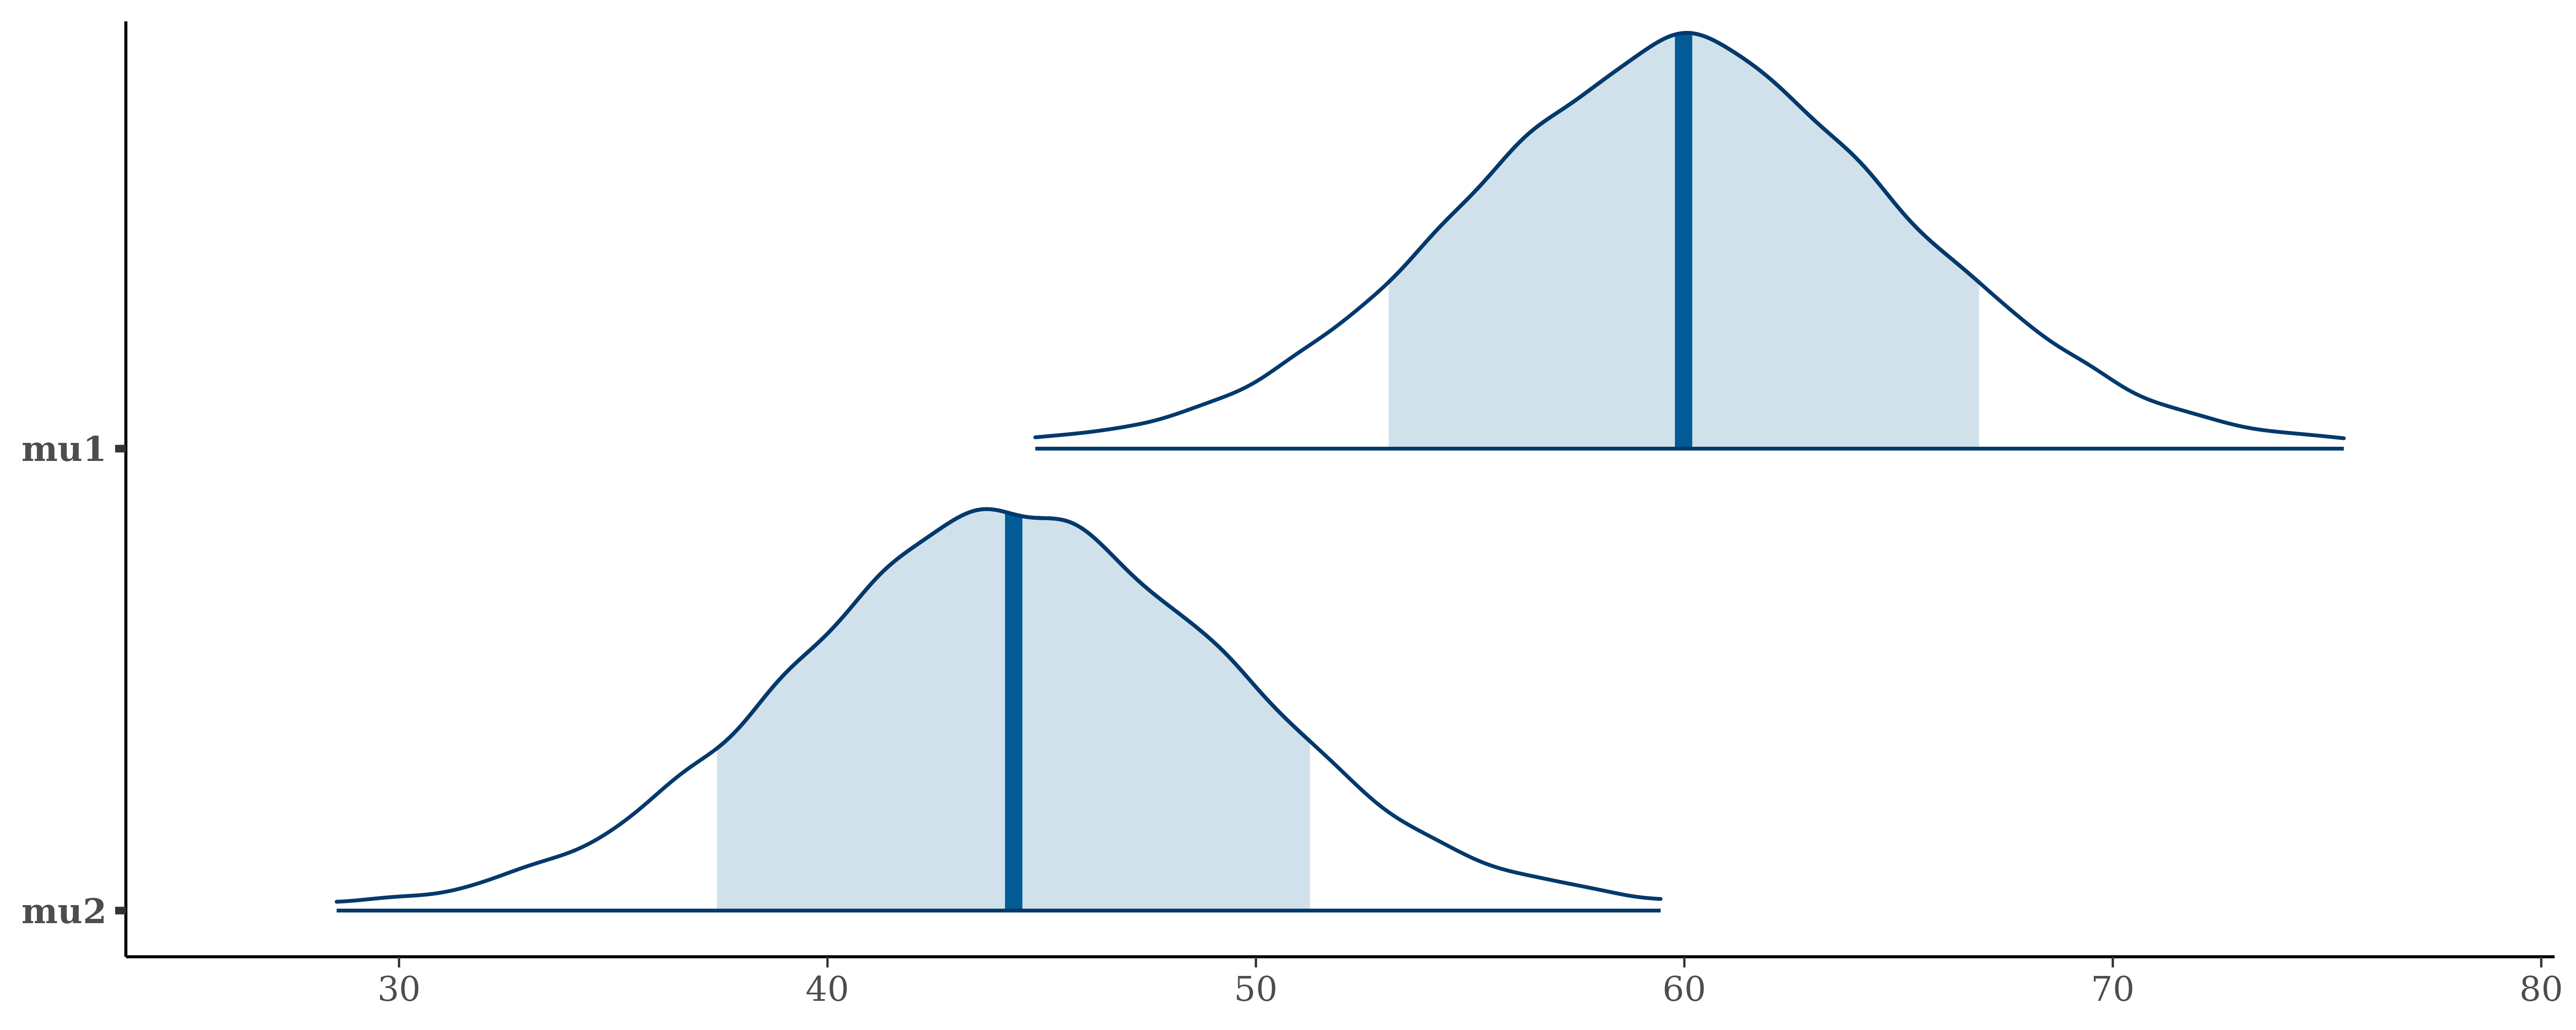
\includegraphics[keepaspectratio,width=12cm]{../images/19_modeling1/Rplot19_01.png}
    \caption{二つの平均値パラメータの事後分布}
    \label{fig::19_02}
\end{figure}
今回は80\%確信区間と，確率分布の両端を99\%のところまで描画してみました。2つの平均値パラメータは，分布の代表値で見ると異なっているのですが，重複している領域が多く一概に「一方が他方より大きい」と言いにくい結果になっています。
帰無仮説検定のようにズバっと「差がある」「ない」と言い切れればいいのですが，このような場合はどうしたらいいでしょうか。

正解は「このままにしておく」です。急いで差があるとかないとか言い切るのではなく，これが区間推定の結果そのものですから，この程度の重複があり得るもの・それほど明確な答えは出ないもの，として考え続けるしかありません。

しかしまあ，このままでは考えるヒントが少ないので，ここで少し工夫をしてみましょう。
帰無仮説検定では，$\mu_A = \mu_B$という帰無仮説が反駁できるかどうかが問題なのでした。今回，$\mu_A$や$\mu_B$を代表する数字の候補が色々ありますので，これを使って「実際どの程度差があったのか」を計算してみれば良いのです。
MCMCサンプルは，毎回推定したいパラメータの同時分布からの代表値を持ってきているという話をしました。例えば1回目のサンプルは$\mu_A = 62.4, \mu_B=25.7$，2回目のサンプルは$\mu_A = 60.4,\,mu_B=36.8$と言った具合に，です。それらは事後分布からのサンプル，事後分布を代表した実現値の1つですから，これを使って$\mu_A - \mu_B$の計算をできます。すると\textbf{差の分布}の代表値がMCMCサンプルで計算できることになります。

これを使って，$\mu_A-\mu_B=0$になる確率はどれぐらいか，というのを考えれば良いのかもしれません。もっとも，連続変数におけるある一点の確率はゼロですし\footnote{確率は相対的な面積で表される数字ですから，面積を持たない点については確率が定義できないのです。}，代表値といってもピッタリゼロになることはほぼあり得ないでしょうから，「どの程度ならゼロと見做すか」ということを考える必要があります。この範囲は\keyterm{実質的に等価な範囲}{じっしつてきにとうかなはんい}{Region Of Practical. Equivalence; ROPE}と呼ばれ，例えばこのテストの例では$\pm5$点ぐらいは誤差みたいなものだけど，5点以上変わったら意味のある違いだ，ということであれば「5点以上点差が出た確率」を計算できます！

この計算は，MCMCサンプルを取り出したRのオブジェクトを使って計算することもできますが，実はStanの中で計算させてしまうこともできます。
\texttt{generated quantities}ブロックが，このMCMCサンプルを取り出したあとの処理をするブロックに該当します。ここで計算される量のことを\keyterm{生成量}{せいせいりょう}{generated quantities}と呼びます。
実際にどのように使うのかをみてみましょう。

\begin{lstlisting}[language=C++,label={stan::19_04},caption={生成量ブロックの利用}]
    ...
generated quantities{
    real diff;
    int<lower=0, upper=1> FLG;
    diff = mu1 - mu2;
    if(diff > 5){
        FLG = 1;
    }else{
        FLG = 0;
    }
}

\end{lstlisting}

コード\ref{stan::19_04}には生成量ブロックを使う例を示しました。ここもブロックですので，変数の宣言が必要です。
今回はまず\verb|diff|という変数を実数型で宣言してみました。これはその下で$\mu_1-\mu_2$として定義されていることからわかるように，差の分布(の代表値)を生成す流のです。これを見ると，差の生じる確率を考えることができます。
次に整数型(int型)で\verb|FLG|という変数を宣言しました。上限が1で下限が0，というか実質的には0か1の数字しか入らない，ある/なし，成立する/しないといった情報しか持たない変数です。いわゆる「フラグが立ったかどうか」の指標であり，その実態は下の\texttt{if}文で表現されています。ここでは先ほど計算した\verb|diff|が5よりも大きいのであれば1，そうでなければ0を代入する，というコードになっています。

これを実行すると，パラメータのサンプルに加えて，そのパラメータから計算されるさまざまな量も同時に算出されます。出力例を見てみましょう。
\begin{SCrstan}{MCMCの結果出力}{out19_02}
    \begin{verbatim}
4 chains, each with iter=5000; warmup=1000; thin=1; 
post-warmup draws per chain=4000, total post-warmup draws=16000.

       mean se_mean   sd   2.5%    25%    50%    75%  97.5% n_eff Rhat
mu1   60.03    0.06 6.72  46.49  55.81  60.09  64.22  73.31 11146    1
mu2   44.29    0.04 4.64  34.99  41.51  44.33  47.10  53.52 11397    1
sig1  18.58    0.06 5.42  11.34  14.84  17.52  21.09  31.92  9700    1
sig2  12.46    0.04 3.69   7.57   9.96  11.71  14.12  21.62  9020    1
diff  15.73    0.08 8.16  -0.19  10.44  15.76  20.95  31.92 10802    1
FLG    0.91    0.00 0.28   0.00   1.00   1.00   1.00   1.00  9978    1
lp__ -50.90    0.02 1.57 -54.86 -51.68 -50.55 -49.74 -48.95  5949    1

Samples were drawn using NUTS(diag_e) at Tue Oct  5 07:46:16 2021.
For each parameter, n_eff is a crude measure of effective sample size,
and Rhat is the potential scale reduction factor on split chains (at 
convergence, Rhat=1). 
   \end{verbatim}
\end{SCrstan}

ここにあるように，差の95\%確信区間は\verb|[-0.19, 31.92]|であることがわかります。差が大きければ31.92，小さければ逆転して-0.19になる可能性すらあるのです。この確信区間は0を含んでいますから，差がない可能性は否定できません。そういう意味で，帰無仮説検定的表現を借りるなら，5\%水準で差がないとは言い切れない，ということができるでしょう。

とはいえ，せっかく分布として情報が得られているのに，点推定にして勝負をするのはもったいないともいえるわけです。結論を急がずに，どの程度の差があるのかをじっくり考えてみるのがいいでしょう。
また変数\verb|FLG|を見ると，その平均が0.91となっています。これは変数\verb|diff|が5よりも大きい時は1，そうでなければ0という条件の数字で，その平均は1になった数を総MCMCサンプル数で割った相対度数になっているのですから，確率を表す数字だと考えても良いことになります。つまり，差が5よりも大きくなる確率は91\%である，と考えることもできるのです。これを応用すると，さまざまな仮説を考えることができそうですね。

\section{帰無仮説検定を省みる}
さてこのように考えてくると，帰無仮説検定について異なる視点で見ることができるようになったのではないでしょうか。ここでは，帰無仮説検定の独特さを3つの点から考えてみたいと思います。
\subsection{不平等な対決}
帰無仮説検定は帰無仮説vs対立仮説という勝負に持ち込んで判断する方法である，ということを冒頭に述べました。
平均値の差の検定の文脈で言えば，帰無仮説は$H0:\mu_1=\mu_2$であり，対立仮説は$H1:\mu_1\neq\mu_2$です。このように，帰無仮説は「差がない」の一点張りであり，対立仮説は「それ以外ならなんでもあり」という状態を指しているのでした。そもそも，帰無仮説というのは非常に限定的な仮説だったのです。無に帰してほしい仮説とは言え，あまりにも不利な勝負なのでした。その上で，勝負は「差がない」「ある」のどちらかにしかなりません。ごく微妙な差であっても，判定によれば差が「あった」といえますし，ギリギリでもなければ「なかった」というしかないのです。このような過度に結果を際立たせる報告は，科学的な研究実践の文脈では拙速なことになりかねませんので，注意が必要なのでした。

データ生成モデリングのやり方で同じデータを分析してみると，差も分布の形で描かれますから，「あったか，なかったか」という単純な問題にせずに色々考えてみたくなるのではないでしょうか。
\subsection{量的な判断を}
もっとも，出力\ref{RS:out19_03}のt検定の結果をよくみてみると，$t$値や$p$値の下に95\%信用区間が示されており，ここでは\verb|[3.570406, 36.429594]|という数字が出ています。そうです，帰無仮説検定をやっているようでも，しっかり区間推定した結果も表示されていたのです。これは差の信用区間で，この区間が0を跨いでいないということは，差がないとは言えない($\mu_A-\mu_B=0$)，ということを意味しています。この区間の幅をみると，3から36と随分ひろくとられているように思えます。つまり，今回の検定結果は差があるとなったけれども，それほど確かなものではないかもしれないぞ，と慎重に判断することもできたはずなのですね。

この差についての量的な評価については，\keyterm{効果量}{こうかりょう}{effect size}という指標で表現されるのでした。効果量とは，標準化された差の大きさです。標準化するというのは，標準偏差で割って幅を整える，あるいは標準偏差何個分という単位で表現することでもあります。比べられるスコアはさまざまですから，その標準偏差で表現することで一般的に議論できるのです。平均値の差の検定においては，\keyterm{Cohenのd}{Cohenのd}{Cohen's d}などが指標としてもいいられますが，それは$\frac{\bar{X}_1-\bar{X}_2}{\sigma}$で計算されるのでした。

これは生成量を使って簡単に計算できます。今回の場合，計算する場合は，生成量に次のようにすれば良いのです。
\begin{lstlisting}[language=C++,label={code::19_06},caption={生成量ブロックで効果量の算出}]
    ...
generated quantities{
    real diff;
    real cohen_d1;
    real cohen_d2;
    diff = mu1 - mu2;
    cohen_d1 = diff / sig1;
    cohen_d2 = diff / sig2;
}

\end{lstlisting}

どちらの群の標準偏差を基準にするか，ということを考える必要がありますが\footnote{二つの標準偏差の平均をとった，プールされた標準偏差で計算することもあります。}，相対的な大きさの比較も簡単にでき，しかもその結果も分布の形で得られる，すなわち効果量の確信区間(効果が少なくともどの程度ありそうかとか，大きければどの程度ありそうかとか)を考えることもできるのです。

もちろんこれらの計算は，帰無仮説検定の文脈，言い換えれば伝統的な統計手法(モーメント法による推論)であってもできたことなのですが，データ生成モデルという観点からみるといっそう理解がしやすいのではないかと思います。
\subsection{方向性を持った仮説も}
今回は最後に，「実験群が統制群よりも5点以上大きくなる確率」というのを考えました。この「一方が他方よりも大きい」という仮説は，帰無仮説検定の文脈では\keyterm{片側検定}{かたがわけんてい}{one-tailed test}と呼ばれます。
一般的に「差がある」という対立仮説は，プラスであれマイナスであれ違いが生じている，という意味であり，統計量は分布の右側でも左側でも，とにかく極端な値になりさえすれば良いという判断でした。
そうではなく「$A>B$のはずだ」という仮定であれば，小さくなる可能性を考えなくていいのですから，統計量のどちらか一方の極について考えれば良いことになります。

とはいえ検定ですから，ある有意水準で一方が他方より大きいと判断すると間違える確率が云々，という判定に落とし込むこという点では同じでした。

今回は生成量を使って，5点以上大きくなる\textbf{確率}を求めることができました。これは検定統計量や$p$値のように架空の値ではなく，もとのデータに直結した数字や確率になっていますから，解釈が比較的自然にできるというのが利点です。
プログラム上の表現も，例えば今回のように\texttt{if}文を使って表現するのは非常に直感的で，「もしあれがこうなってそれがこうなったらどうなる？」といろいろな仮説を考えていくこともできますね。
帰無仮説検定のロジックは，結果判定のために仮説を限定的な型にはめ込んでしまいます。しかしその型を飛び越えていろいろなことをやってもいいのだ，できるんだというのは，データがどうやって生まれてきているかを考えている「創造主」としての特権かもしれません。

ただし注意してもらいたいのは，これらの検証の仕方は，今回のデータと仮定されたモデルという前提の上で成立する割合を確立とみなしているに過ぎない，ということです。データが変わればその数字も変わるでしょうし，そもそもデータが正規分布から出てきていないのかもしれません。本当はXX分布から出てきているのに，YY分布を仮定したモデルで計算したら，仮説が正しい可能性が100\% !といっても虚しい(明らかに間違っている)ことになりますね。心理学のデータの場合はえてして，どういう分布やメカニズムになるのかがはっきりわからないものです。ただ，あまりにもわからなさ過ぎて，さまざまな影響が混ぜ合わさっているので，色んな要素が相殺しあって結局ほとんど正規分布とみなしていいよ，ということだったりします。心という目に見えないものに，不良設定問題を解くためのツールで立ち向かうという，無理に無理を重ねるような推論の世界であるということに，自覚は持っていたいですね\footnote{いいんです，それでも。だってそんなよくわからない人間というのが好きなんですから。}。


\section{今回のまとめ}
我々がデータを分析する時は，そのデータの数字がどうであったか，ということを真っ先に考えたいはずです。身長の差は何センチあったのか，最終学歴によって生涯年収は何円差がつくのか，といった具体的な単位に基づく\textbf{実質的な差}が一番大事なはずです。
心理学をやっていくと，尺度をはじめとした「絶対的なスコア」が出てきませんから，尺度で何ポイント差があったのか，ということがあまり意味のある実態と対応しないことも少なくありません。そう言った時のために，\textbf{標準化された差}を考えるようになったのです。その計算は非常に面倒ですが，機械がすぐに計算してくれることによって結論を急ぎすぎ，単位も実際のデータとも関係のない統計量を参照して\textbf{有意差}を求めるようになってしまったのでは意味がありません。

データがどういうメカニズムで生まれてきたかを考え，母数をベイズ推定するというやり方は，いちいちコードを書かなければならないこともあって，非常に手間がかかるようにも思えます。しかし自分が何を仮定していたのか，どういうメカニズムの元で考えていたのかを自覚し，またその推定値を使って自由に仮説を考えることで，決まりきった分析手続きに落とし込むという単調な作業から解放され，クリエイティブにデータに向き合えることでもあります。
\section{課題}
次の計算をするR/Stanコードや回答を記述し，提出してください。なお提出されたコード単体でバグがなく動くことが確認できないものは，未提出扱いになります。コードの書き方などわからないところがあれば，曜日別TAか小杉までメールで連絡し，指導を受けてください。

\paragraph{フライドポテトの研究}
あるコンビニで，ホットスナックのフレンチフライを2つ買ったところ，どうも一方より他方の方が長くて大きい気がした。そこでそれぞれの袋から取り出して長さを測定してみた(単位cm)。測定結果が表\ref{tab::19_01}である\footnote{このデータは実際に筆者がコンビニの二つの店舗でポテトを購入し，長さを測定した結果に基づいています。}。
\begin{table}[ht]
    \center
    \caption{二つの店舗のポテトの長さ}
\begin{tabular}{c|cccccccccccccccccc}\hline
    A & 8.4 & 11.3 & 8.1 & 11.2 & 5.8 & 6.3 & 7.1 & 10.9 & 7.1 & 6.5 & 5.0 & 3.0 & 7.2 & 6.5 & 6.4 & 6.4 & 9.3 & 8.3 \\\hline
    B & 6.7 & 7.2 & 4.2 & 11.0 & 7.5 & 8.9 & 7.0 & 8.0 & 7.2 & 4.2 & 6.0 & 9.0 & 8.6 & 9.0 & 5.0 &  &  &  \\\hline
\end{tabular}
\label{tab::19_01}
\end{table}
このデータを用いて次の問に答えなさい。なおこの数値はサイト上のコードで取得可能です。
\begin{enumerate}
    \item ポテトの長さは正規分布に従うと仮定します。また両群の分布の幅は同じであると仮定します。t検定で二群の平均値に差があるかどうか，判断してください。t値や自由度，p値を参照しながら説明すること。効果量も算出するとなお良いです。
    \item ポテトの長さは正規分布に従うと仮定します。また両群の分布の幅は同じであると仮定します。その上で，群Aと群Bの平均値を推定するモデルを作り，ベイズ推定してください。その上で，結果の平均値，中央値，MAP推定値，90\%確信区間を報告してください。
    \item 両群のポテトの長さの平均が，3cm以上違うようであればクレームをつけに行こうと思います。3cm以上の差がある確率はどれぐらいですか。推定してください。
    \item よく考えてみれば，両郡の分布の幅が同じであるという仮定はおかしいような気がしてきました。そこで，それぞれの群毎に分布の幅を推定するモデルに作り替え，ベイズ推定してください。その上で，結果の平均値，中央値，MAP推定値，90\%確信区間を報告推定してください
    \item 異なる分散を指定したモデルで，両群のポテトの長さの平均差が5cm以内であれば，クレームをつけにいくのはやめておこうと思います。差が5cm以内である確率はどれぐらいですか。推定してください。
\end{enumerate}
\end{document} 
